% GENERATED FILE - do not hand-edit.
% Source of truth: data/calculus-reviewed/c-8.json in the zenith-website repo.
% Regenerate with: python3 scripts/build_calculus_tex.py
\documentclass[11pt]{article}
\usepackage[utf8]{inputenc}
\usepackage[T1]{fontenc}
\usepackage{amsmath,amssymb}
\usepackage{graphicx}
\usepackage[margin=1in]{geometry}
\graphicspath{{../..//}}
\setlength{\parindent}{0pt}
\setlength{\parskip}{0.6em}
\begin{document}
\section*{Chapter 8: Further Applications of Integration --- Practice Exercises C8}

\bigskip\noindent\textbf{A1.}\ A particle has position $s(t)=t^3-6t^2+9t+3$. When does its direction change?
\begin{list}{}{\setlength{\leftmargin}{3em}\setlength{\labelwidth}{2.5em}\setlength{\itemsep}{0pt}\setlength{\topsep}{2pt}}
\item[(A)] $t=1$ only
\item[(B)] $t=2$ only
\item[(C)] $t=3$ only
\item[(D)] $t=1$ and $t=3$
\end{list}

\bigskip\noindent\textbf{A2.}\ A body's velocity is $v=4t^3+3t^2+5$. Find its distance traveled from $t=0$ to $t=2$.
\begin{list}{}{\setlength{\leftmargin}{3em}\setlength{\labelwidth}{2.5em}\setlength{\itemsep}{0pt}\setlength{\topsep}{2pt}}
\item[(A)] $34$
\item[(B)] $49$
\item[(C)] $24$
\item[(D)] $44$
\end{list}

\bigskip\noindent\textbf{A3.}\ A particle has velocity $v=3t^2-6t$. Find total distance traveled from $t=0$ to $t=3$.
\begin{list}{}{\setlength{\leftmargin}{3em}\setlength{\labelwidth}{2.5em}\setlength{\itemsep}{0pt}\setlength{\topsep}{2pt}}
\item[(A)] $0$
\item[(B)] $4$
\item[(C)] $8$
\item[(D)] $9$
\end{list}

\bigskip\noindent\textbf{A4.}\ A particle has velocity $v(t)=3t^2-6t$. Find its net position change from $t=0$ to $t=3$.
\begin{list}{}{\setlength{\leftmargin}{3em}\setlength{\labelwidth}{2.5em}\setlength{\itemsep}{0pt}\setlength{\topsep}{2pt}}
\item[(A)] $0$
\item[(B)] $4$
\item[(C)] $8$
\item[(D)] $9$
\end{list}

\bigskip\noindent\textbf{A5.}\ A particle has acceleration $a=\cos t$ and is at rest at $t=0$. Find its distance traveled from $t=0$ to $t=2$.
\begin{list}{}{\setlength{\leftmargin}{3em}\setlength{\labelwidth}{2.5em}\setlength{\itemsep}{0pt}\setlength{\topsep}{2pt}}
\item[(A)] $\sin2$
\item[(B)] $1-\cos2$
\item[(C)] $2-\sin2$
\item[(D)] $-\cos2$
\end{list}

\bigskip\noindent\textbf{A6.}\ A hurricane's wind velocity is $v(t)=5t-t^2+100$ mph for $0\le t\le4$ hours. Find average wind velocity over this period.
\begin{list}{}{\setlength{\leftmargin}{3em}\setlength{\labelwidth}{2.5em}\setlength{\itemsep}{0pt}\setlength{\topsep}{2pt}}
\item[(A)] $100$
\item[(B)] $102$
\item[(C)] $104\tfrac23$
\item[(D)] $108\tfrac23$
\end{list}

\bigskip\noindent\textbf{A7.}\ An object has acceleration $\vec a(t)=\langle2t,e^t\rangle$ and initial velocity $\vec v(0)=\langle2,0\rangle$. Find $\vec v(t)$.
\begin{list}{}{\setlength{\leftmargin}{3em}\setlength{\labelwidth}{2.5em}\setlength{\itemsep}{0pt}\setlength{\topsep}{2pt}}
\item[(A)] $\langle t^2,e^t+1\rangle$
\item[(B)] $\langle t^2+2,e^t\rangle$
\item[(C)] $\langle t^2+2,e^t-1\rangle$
\item[(D)] $\langle2,e^t-1\rangle$
\end{list}

\bigskip\noindent\textbf{A8.}\ A stone is thrown upward from ground level at $96$ ft/sec, with $a(t)=-32$ ft/sec$^2$. Find its average velocity during the first two seconds.
\begin{list}{}{\setlength{\leftmargin}{3em}\setlength{\labelwidth}{2.5em}\setlength{\itemsep}{0pt}\setlength{\topsep}{2pt}}
\item[(A)] $16$ ft/sec
\item[(B)] $32$ ft/sec
\item[(C)] $64$ ft/sec
\item[(D)] $80$ ft/sec
\end{list}

\bigskip\noindent\textbf{A9.}\ On the 20-mile highway stretch south of a bridge, vehicle density is $f(x)$ cars/mile at distance $x$ miles south. Which expression gives the number of cars from the bridge to a point $x$ miles south?
\begin{list}{}{\setlength{\leftmargin}{3em}\setlength{\labelwidth}{2.5em}\setlength{\itemsep}{0pt}\setlength{\topsep}{2pt}}
\item[(A)] $\int_0^xf(t)\,dt$
\item[(B)] $\int_x^{20}f(t)\,dt$
\item[(C)] $\int_0^{20}f(x)\,dx$
\item[(D)] $\sum_{k=1}^nf(x_k)\Delta x$, using $n$ equal subdivisions of the entire 20-mile stretch
\end{list}

\bigskip\noindent\textbf{A10.}\ A circular city has radius 3 miles, and a straight highway runs along a diameter. Density at distance $x$ miles from the highway is $f(x)=12-2x$ thousand people per square mile. Which integral gives its population in thousands?
\begin{list}{}{\setlength{\leftmargin}{3em}\setlength{\labelwidth}{2.5em}\setlength{\itemsep}{0pt}\setlength{\topsep}{2pt}}
\item[(A)] $\int_0^3(12-2x)\,dx$
\item[(B)] $2\int_0^3(12-2x)\sqrt{9-x^2}\,dx$
\item[(C)] $4\int_0^3(12-2x)\sqrt{9-x^2}\,dx$
\item[(D)] $\int_0^3 2\pi x(12-2x)\,dx$
\end{list}

\bigskip\noindent\textbf{B1.}\ A car accelerates constantly from 0 to 60 mph in 10 seconds. Given 60 mph = 88 ft/sec, find acceleration in ft/sec$^2$.
\begin{list}{}{\setlength{\leftmargin}{3em}\setlength{\labelwidth}{2.5em}\setlength{\itemsep}{0pt}\setlength{\topsep}{2pt}}
\item[(A)] $1.76$
\item[(B)] $5.3$
\item[(C)] $6$
\item[(D)] $8.8$
\end{list}

\bigskip\noindent\textbf{B2.}\ A particle has velocity $\mathbf v(t)=\langle t,t-1\rangle$ and initial position $(0,1)$. Find its position vector at time $t$.
\begin{list}{}{\setlength{\leftmargin}{3em}\setlength{\labelwidth}{2.5em}\setlength{\itemsep}{0pt}\setlength{\topsep}{2pt}}
\item[(A)] $\langle t^2/2,-(1-t^2)/2\rangle$
\item[(B)] $\langle t^2/2,-(1-t^2)/2\rangle$
\item[(C)] $\langle t^2/2,-(t^2-2t)/2\rangle$
\item[(D)] $\langle t^2/2,(t^2-2t+2)/2\rangle$
\end{list}

\bigskip\noindent\textbf{B3.}\ A particle has velocity $\mathbf v(t)=\langle t,t-1\rangle$ and initial position $(0,1)$. Find its acceleration at $t=2$.
\begin{list}{}{\setlength{\leftmargin}{3em}\setlength{\labelwidth}{2.5em}\setlength{\itemsep}{0pt}\setlength{\topsep}{2pt}}
\item[(A)] $\langle1,1\rangle$
\item[(B)] $\langle1,-1\rangle$
\item[(C)] $\langle1,2\rangle$
\item[(D)] $\langle2,-1\rangle$
\end{list}

\bigskip\noindent\textbf{B4.}\ A particle has velocity $\mathbf v(t)=\langle t,t-1\rangle$ and initial position $(0,1)$. When is its speed minimized?
\begin{list}{}{\setlength{\leftmargin}{3em}\setlength{\labelwidth}{2.5em}\setlength{\itemsep}{0pt}\setlength{\topsep}{2pt}}
\item[(A)] $0$
\item[(B)] $1/2$
\item[(C)] $1$
\item[(D)] $1.5$
\end{list}

\bigskip\noindent\textbf{B5.}\ A particle's position and velocity vectors are perpendicular at all times. It passes through $(4,3)$. Find the equation of its curve.
\begin{list}{}{\setlength{\leftmargin}{3em}\setlength{\labelwidth}{2.5em}\setlength{\itemsep}{0pt}\setlength{\topsep}{2pt}}
\item[(A)] $x^2+y^2=5$
\item[(B)] $x^2+y^2=25$
\item[(C)] $x^2+2y^2=34$
\item[(D)] $x^2-y^2=7$
\end{list}

\bigskip\noindent\textbf{B6.}\ An object has velocity $\vec v(t)=\langle3\sqrt t,4\rangle$ and is at the origin at $t=1$. Where was it at $t=0$?
\begin{list}{}{\setlength{\leftmargin}{3em}\setlength{\labelwidth}{2.5em}\setlength{\itemsep}{0pt}\setlength{\topsep}{2pt}}
\item[(A)] $(-2,-4)$
\item[(B)] $(2,4)$
\item[(C)] $(3/2,0)$
\item[(D)] $(-3/2,0)$
\end{list}

\bigskip\noindent\textbf{B7.}\ World population is modeled by $P(t)=8e^{0.0105t}$ billion, $t$ years from now. Find average population over the next 25 years.
\begin{list}{}{\setlength{\leftmargin}{3em}\setlength{\labelwidth}{2.5em}\setlength{\itemsep}{0pt}\setlength{\topsep}{2pt}}
\item[(A)] $8.096$
\item[(B)] $8.197$
\item[(C)] $8.827$
\item[(D)] $9.148$
\end{list}

\bigskip\noindent\textbf{B8.}\ A beach opens at 8 A.M. and people arrive at $R(t)=10+40t$ people/hour, where $t$ is hours after opening. No one leaves before noon. When will 100 people be there?
\begin{list}{}{\setlength{\leftmargin}{3em}\setlength{\labelwidth}{2.5em}\setlength{\itemsep}{0pt}\setlength{\topsep}{2pt}}
\item[(A)] 9:45
\item[(B)] 10:00
\item[(C)] 10:15
\item[(D)] 10:30
\end{list}

\bigskip\noindent\textbf{B9.}\ A drug amount is $A(t)=30/(t+1)^2$ mg at $t$ hours. Find average amount during the first four hours.
\begin{list}{}{\setlength{\leftmargin}{3em}\setlength{\labelwidth}{2.5em}\setlength{\itemsep}{0pt}\setlength{\topsep}{2pt}}
\item[(A)] $6.0$ mg
\item[(B)] $11.0$ mg
\item[(C)] $16.6$ mg
\item[(D)] $24.0$ mg
\end{list}

\bigskip\noindent\textbf{B10.}\ A rumor spreads at $R(t)=t^2+10t$ new people/day, $t$ days after first heard. Approximately how many people hear it during the second week, from day 7 to day 14?
\begin{list}{}{\setlength{\leftmargin}{3em}\setlength{\labelwidth}{2.5em}\setlength{\itemsep}{0pt}\setlength{\topsep}{2pt}}
\item[(A)] $359$
\item[(B)] $1535$
\item[(C)] $1894$
\item[(D)] $2219$
\end{list}

\bigskip\noindent\textbf{B11.}\ Oil leaks at $L(t)=1000e^{-0.3t}$ gallons/hour. Approximately how many gallons leak in the first 8 hours?
\begin{list}{}{\setlength{\leftmargin}{3em}\setlength{\labelwidth}{2.5em}\setlength{\itemsep}{0pt}\setlength{\topsep}{2pt}}
\item[(A)] $1271$
\item[(B)] $3031$
\item[(C)] $3161$
\item[(D)] $4323$
\end{list}

\bigskip\noindent\textbf{B12.}\ City population density at distance $x$ from the center is given by $\begin{array}{c|rrrrrr}x\text{ (miles)}&0&2&4&6&8&10\\\hline f(x)\text{ (hundreds per square mile)}&50&45&40&30&15&5\end{array}$. Use a left Riemann sum to estimate population within a 10-mile radius.
\begin{list}{}{\setlength{\leftmargin}{3em}\setlength{\labelwidth}{2.5em}\setlength{\itemsep}{0pt}\setlength{\topsep}{2pt}}
\item[(A)] $36{,}000$
\item[(B)] $226{,}200$
\item[(C)] $691{,}200$
\item[(D)] $754{,}000$
\end{list}

\bigskip\noindent\textbf{B13.}\ A factory dumps pollutants at $P(t)=\sqrt t/180$ tons/day. Approximately how much is dumped after 7 weeks?
\begin{list}{}{\setlength{\leftmargin}{3em}\setlength{\labelwidth}{2.5em}\setlength{\itemsep}{0pt}\setlength{\topsep}{2pt}}
\item[(A)] $0.07$ ton
\item[(B)] $0.90$ ton
\item[(C)] $1.55$ tons
\item[(D)] $1.27$ tons
\end{list}

\bigskip\noindent\textbf{B14.}\ A roast initially at $160^\circ$F is put in a $45^\circ$F refrigerator. Its temperature changes at $R(t)=-9e^{-0.08t}$ degrees F/minute. Find its temperature after 20 minutes, to the nearest degree.
\begin{list}{}{\setlength{\leftmargin}{3em}\setlength{\labelwidth}{2.5em}\setlength{\itemsep}{0pt}\setlength{\topsep}{2pt}}
\item[(A)] $45^\circ$
\item[(B)] $70^\circ$
\item[(C)] $81^\circ$
\item[(D)] $90^\circ$
\end{list}

\bigskip\noindent\textbf{B15.}\ Pollutant is released at $P(t)=te^{-0.3t}$ tons/week. How long does it take to release 9 tons?
\begin{list}{}{\setlength{\leftmargin}{3em}\setlength{\labelwidth}{2.5em}\setlength{\itemsep}{0pt}\setlength{\topsep}{2pt}}
\item[(A)] $10.2$ weeks
\item[(B)] $11.0$ weeks
\item[(C)] $12.1$ weeks
\item[(D)] $12.9$ weeks
\end{list}

\bigskip\noindent\textbf{B16.}\ Find the total area between $f(x)=x^3-4x^2+3x$ and the $x$-axis on $[0,3]$.
\begin{list}{}{\setlength{\leftmargin}{3em}\setlength{\labelwidth}{2.5em}\setlength{\itemsep}{0pt}\setlength{\topsep}{2pt}}
\item[(A)] $-2.25$
\item[(B)] $2.25$
\item[(C)] $3$
\item[(D)] $3.083$
\end{list}

\bigskip\noindent\textbf{B17.}\ Water leaks at $W(t)=-0.1t^2-0.3t+2$ gallons/hour. Find the total amount that leaks in the next 3 hours.
\begin{list}{}{\setlength{\leftmargin}{3em}\setlength{\labelwidth}{2.5em}\setlength{\itemsep}{0pt}\setlength{\topsep}{2pt}}
\item[(A)] $2.08$
\item[(B)] $3.13$
\item[(C)] $3.48$
\item[(D)] $3.75$
\end{list}

\bigskip\noindent\textbf{B18.}\ A culture grows at $B(t)=1000e^{0.03t}$ bacteria/hour. Find its total increase during the second hour.
\begin{list}{}{\setlength{\leftmargin}{3em}\setlength{\labelwidth}{2.5em}\setlength{\itemsep}{0pt}\setlength{\topsep}{2pt}}
\item[(A)] $1015$
\item[(B)] $1046$
\item[(C)] $1061$
\item[(D)] $1077$
\end{list}

\bigskip\noindent\textbf{B19.}\ A website opens at noon. The graph gives its increasing visitor rate $R(t)$ in visitors/hour over the next 8 hours. Use a midpoint or trapezoidal sum to estimate when the 200th visitor arrives.
\begin{center}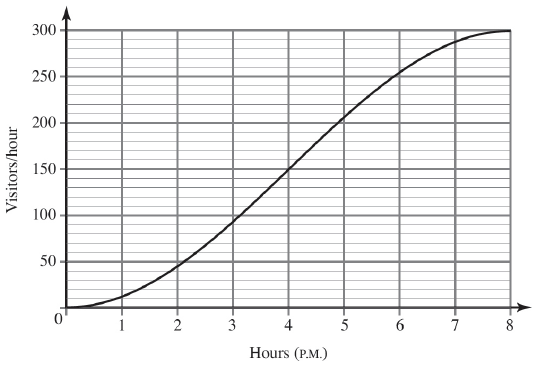
\includegraphics[width=0.6\linewidth]{data/calculus-figures/c8-b19.png}\end{center}
\begin{list}{}{\setlength{\leftmargin}{3em}\setlength{\labelwidth}{2.5em}\setlength{\itemsep}{0pt}\setlength{\topsep}{2pt}}
\item[(A)] Between 2 and 3 P.M.
\item[(B)] Between 3 and 4 P.M.
\item[(C)] Between 4 and 5 P.M.
\item[(D)] After 5 P.M.
\end{list}

\bigskip\noindent\textbf{B20.}\ Velocity observations are $\begin{array}{c|rrrrrr}t\text{ (sec)}&0&2&3&5&7&10\\\hline v(t)\text{ (units/sec)}&2&3&1&-1&-2&0\end{array}$. Use the five indicated trapezoids to estimate how far from its starting point the object comes to rest at $t=10$.
\begin{list}{}{\setlength{\leftmargin}{3em}\setlength{\labelwidth}{2.5em}\setlength{\itemsep}{0pt}\setlength{\topsep}{2pt}}
\item[(A)] $0$ units
\item[(B)] $1$ unit
\item[(C)] $3$ units
\item[(D)] $4$ units
\end{list}

\bigskip\noindent\textbf{B21.}\ A truck travels at $v(t)=80(t+1)/(t+2)$ mph, $t$ hours after starting. Fuel economy is $f(v)=4+0.01v$ miles/gallon. Find gallons consumed in the first two hours.
\begin{list}{}{\setlength{\leftmargin}{3em}\setlength{\labelwidth}{2.5em}\setlength{\itemsep}{0pt}\setlength{\topsep}{2pt}}
\item[(A)] $20$
\item[(B)] $21.5$
\item[(C)] $23.1$
\item[(D)] $24$
\end{list}

\end{document}
